\begin{samepage}

\begin{table}[h]
\centering
\renewcommand{\arraystretch}{1.2}
\caption[Counterfactuals for various masking methods]{Examples of counterfactual explanations across different masking methods. Each block shows original image, masked variant, reconstructed image, and final prediction.}
\label{tab:cf_masking_comparison}

\begin{tabular}{c|c|c|c}
\textbf{Input Image} & 
\makecell[c]{\textbf{Grid-Based} \\ \textbf{Masking}} & 
\makecell[c]{\textbf{Object Detection} \\ \textbf{Based Masking}} & 
\makecell[c]{\textbf{LIME on Image} \\ \textbf{Based Masking}} \\
\toprule

% ---------- Row 1 ----------
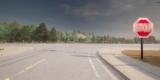
\includegraphics[width=0.18\textwidth]{img/appendix/original_town7_000980.png} &
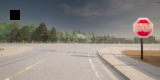
\includegraphics[width=0.18\textwidth]{img/appendix/grid_masked_town7_000980.png} &
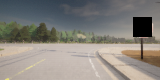
\includegraphics[width=0.18\textwidth]{img/appendix/object_masked_town7_000980.png} &
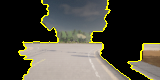
\includegraphics[width=0.18\textwidth]{img/appendix/LIME_on_Image_maksed_town7_000980.png} \\

\textcolor{red}{STOP} &
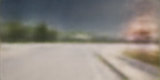
\includegraphics[width=0.18\textwidth]{img/appendix/grid_reconstructed_town7_000980.png} &
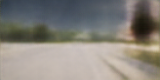
\includegraphics[width=0.18\textwidth]{img/appendix/object_reconstructed_town7_000980.png} &
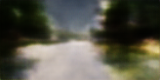
\includegraphics[width=0.18\textwidth]{img/appendix/LIME_on_Image_reconstructed_town7_000980.png} \\

& \textcolor{green}{GO} & \textcolor{green}{GO} & \textcolor{blue}{RIGHT} \\

\midrule

% ---------- Row 2 ----------
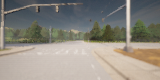
\includegraphics[width=0.18\textwidth]{img/appendix/original_town7_000919.png} &
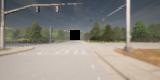
\includegraphics[width=0.18\textwidth]{img/appendix/grid_masked_town7_000919.png} &
\makecell[c]{\footnotesize Failed to \\ \footnotesize detect object} &
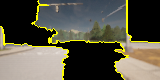
\includegraphics[width=0.18\textwidth]{img/appendix/LIME_on_Image_maksed_town7_000919.png} \\

\textcolor{green}{GO} &
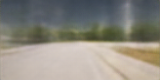
\includegraphics[width=0.18\textwidth]{img/appendix/grid_reconstructed_town7_000919.png} &
-- &
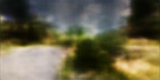
\includegraphics[width=0.18\textwidth]{img/appendix/LIME_on_Image_reconstructed_town7_000919.png} \\

& \textcolor{blue}{RIGHT} & \textcolor{red}{--} & \textcolor{red}{STOP} \\

\midrule

% ---------- Row 3 ----------
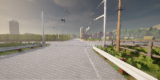
\includegraphics[width=0.18\textwidth]{img/appendix/original_town7_010910.png} &
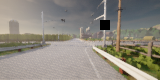
\includegraphics[width=0.18\textwidth]{img/appendix/grid_masked_town7_010910.png} &
\makecell[c]{\footnotesize Failed to \\ \footnotesize detect object} &
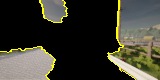
\includegraphics[width=0.18\textwidth]{img/appendix/LIME_on_Image_maksed_town7_010910.png} \\

\textcolor{green}{GO} &
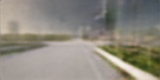
\includegraphics[width=0.18\textwidth]{img/appendix/grid_reconstructed_town7_010910.png} &
-- &
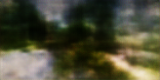
\includegraphics[width=0.18\textwidth]{img/appendix/LIME_on_Image_reconstructed_town7_010910.png} \\

& \textcolor{teal}{LEFT} & \textcolor{red}{--} & \textcolor{red}{STOP} \\

\bottomrule

\end{tabular}
\end{table}
\end{samepage}



\clearpage

\begin{table}[htbp]
\centering
\renewcommand{\arraystretch}{1.2}
\caption[LIME + NUN counterfactual examples]{Examples of successful counterfactual explanations using LIME-guided latent masking and Nearest Unlike Neighbor (NUN) method. Original label and new prediction after reconstruction are indicated.}
\label{tab:cf_nun_lime_examples}
\begin{tabular}{c|c|c}
\textbf{Original Image} & \textbf{LIME on Latent feature} & \textbf{LIME on Latent using NUN} \\
\toprule

% ---------- Row 1 ----------
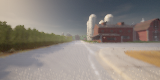
\includegraphics[width=0.18\textwidth]{img/appendix/original_town7_011020.png} &
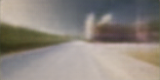
\includegraphics[width=0.18\textwidth]{img/appendix/latent_recon_town7_011020.png} &
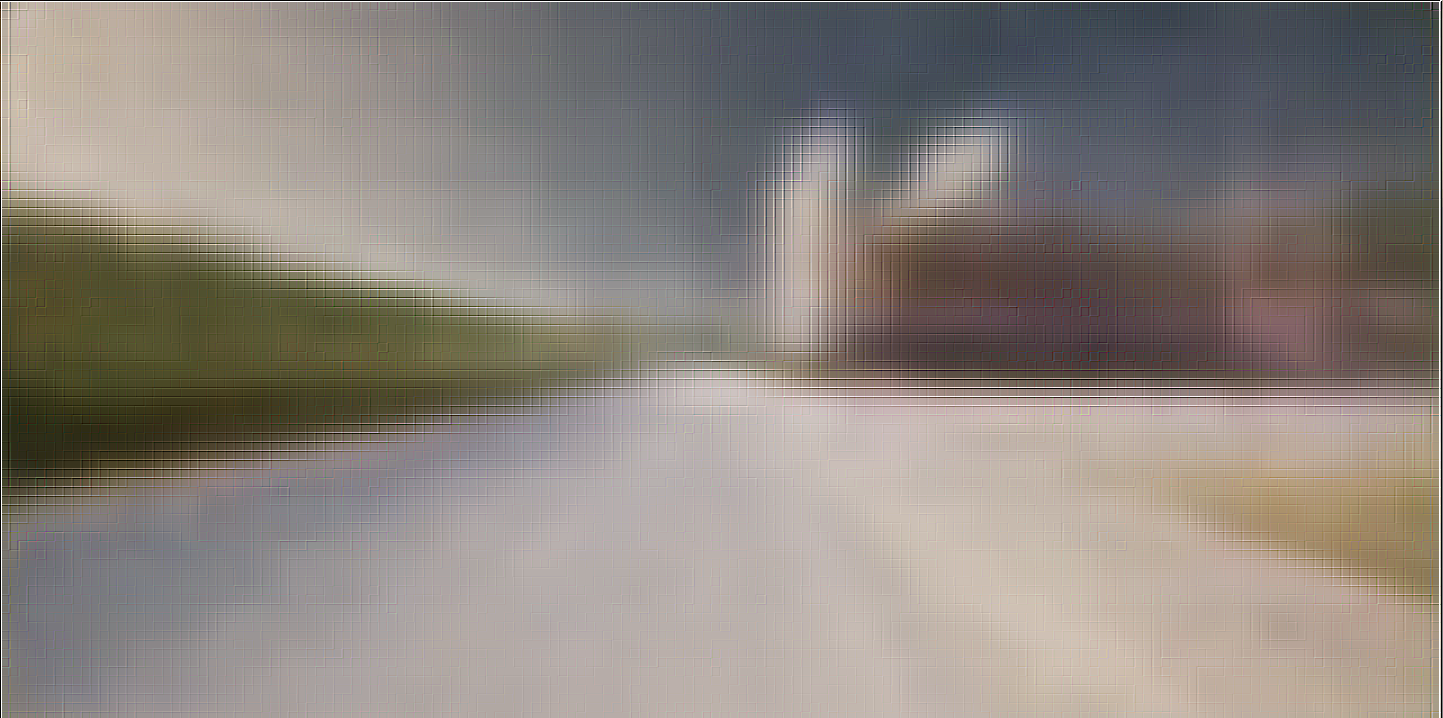
\includegraphics[width=0.18\textwidth]{img/appendix/nun_recon_town7_011020.png} \\
\textcolor{green}{GO}  & 
\textcolor{green}{GO} $\rightarrow$ \textcolor{blue}{RIGHT} & 
\textcolor{green}{GO} $\rightarrow$ \textcolor{blue}{RIGHT} \\
\midrule

% ---------- Row 2 ----------
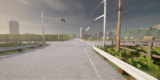
\includegraphics[width=0.18\textwidth]{img/appendix/original_town7_010880.png} &
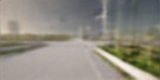
\includegraphics[width=0.18\textwidth]{img/appendix/latent_recon_town7_010880.png} &
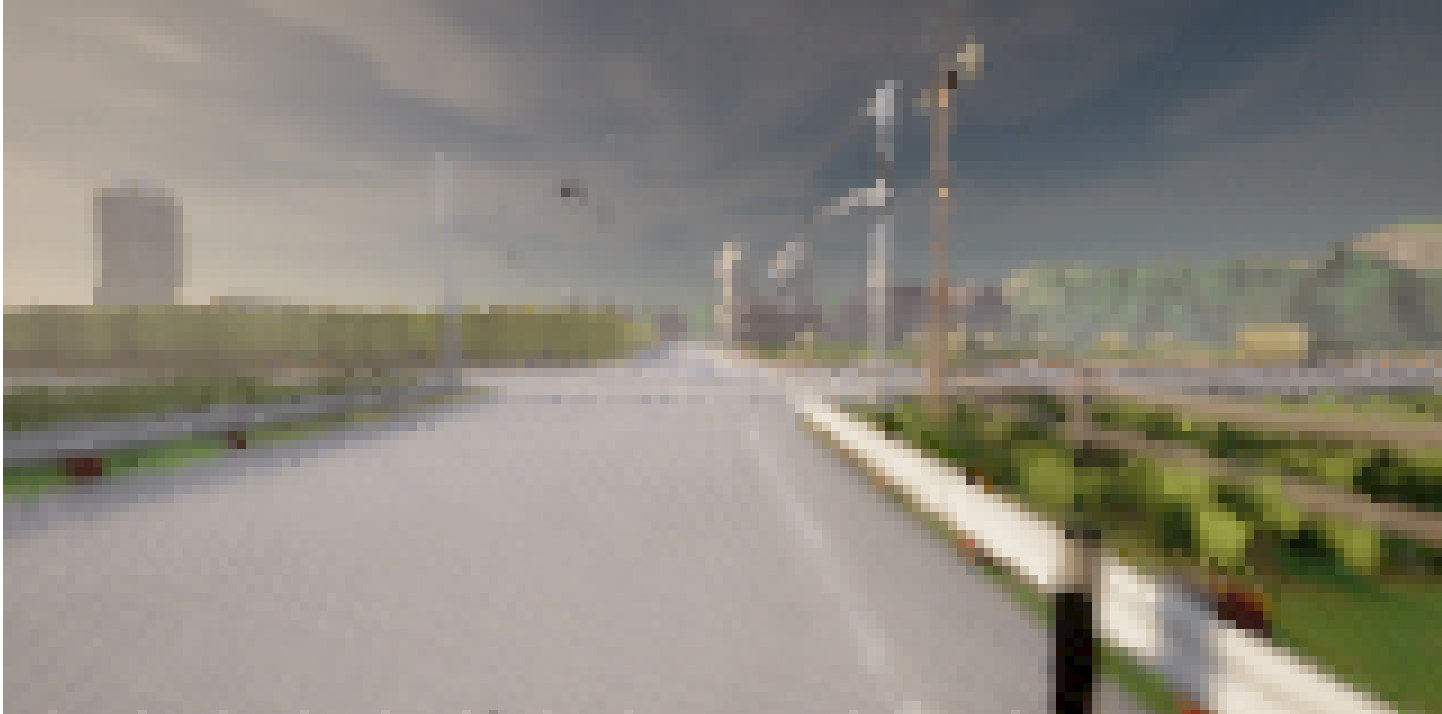
\includegraphics[width=0.18\textwidth]{img/appendix/nun_recon_town7_010880.png} \\
\textcolor{red}{STOP}  & 
\textcolor{red}{STOP} $\rightarrow$ \textcolor{blue}{RIGHT} & 
\textcolor{red}{STOP} $\rightarrow$ \textcolor{blue}{RIGHT} \\
\midrule

% ---------- Row 3 ----------
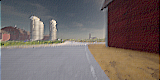
\includegraphics[width=0.18\textwidth]{img/appendix/original_town7_005399.png} &
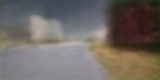
\includegraphics[width=0.18\textwidth]{img/appendix/latent_recon_town7_005399.png} &
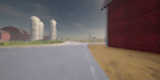
\includegraphics[width=0.18\textwidth]{img/appendix/nun_recon_town7_005399.png} \\
\textcolor{green}{GO}  & 
\textcolor{green}{GO} $\rightarrow$ \textcolor{red}{STOP} & 
\textcolor{green}{GO} $\rightarrow$ \textcolor{teal}{LEFT} \\
\midrule

% ---------- Row 4 ----------
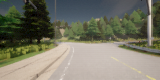
\includegraphics[width=0.18\textwidth]{img/appendix/original_town001.png} &
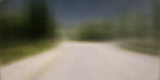
\includegraphics[width=0.18\textwidth]{img/appendix/recon_latent.png} &
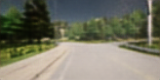
\includegraphics[width=0.18\textwidth]{img/appendix/recon_nun.png} \\
\textcolor{teal}{LEFT}  & 
\textcolor{teal}{LEFT} $\rightarrow$ \textcolor{red}{STOP} & 
\textcolor{teal}{LEFT} $\rightarrow$ \textcolor{green}{GO} \\

\bottomrule

\end{tabular}
\end{table}




